\subsection{Results of the supervised approach} \label{results_supervised}

\begin{figure}
  \begin{subfigure}[t]{.5\textwidth}
    \centering
    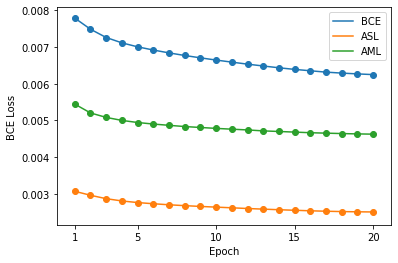
\includegraphics[width=\textwidth]{figures/supervised_approach/all_train_loss.png}
    \caption{Training loss}
    \label{fig:all_train_loss}
  \end{subfigure}
   \begin{subfigure}[t]{.5\textwidth}
    \centering
    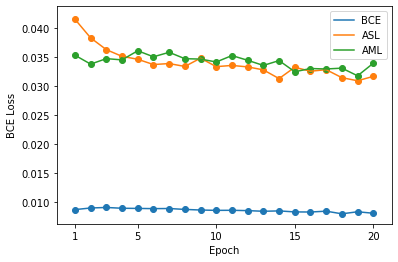
\includegraphics[width=\textwidth]{figures/supervised_approach/all_test_loss.png}
    \caption{Testing loss}
    \label{fig:all_test_loss}
  \end{subfigure}
  \caption{Test and training loss of the three final models.}
  \label{fig:all_train}
\end{figure}

\begin{figure}
  \begin{subfigure}[t]{.32\textwidth}
    \centering
    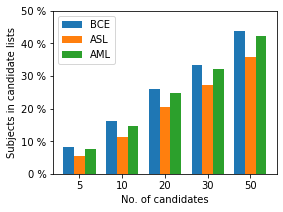
\includegraphics[width=\textwidth]{figures/supervised_approach/all_hw.png}
    \caption{Handwritten subjects}
    \label{fig:all_hw}
  \end{subfigure}
  \begin{subfigure}[t]{.32\textwidth}
    \centering
    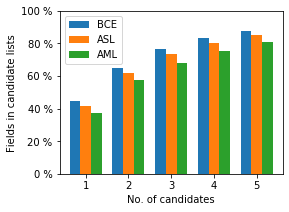
\includegraphics[width=\textwidth]{figures/supervised_approach/all_ddc.png}
    \caption{DDC subjects}
    \label{fig:all_ddc}
  \end{subfigure}
   \begin{subfigure}[t]{.32\textwidth}
    \centering
    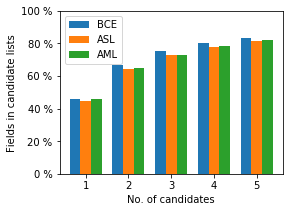
\includegraphics[width=\textwidth]{figures/supervised_approach/all_venue.png}
    \caption{Venues}
    \label{fig:all_venue}
  \end{subfigure}
  \caption{Hit rate of the three final models for the evaluation sets.}
  \label{fig:all_eval}
\end{figure}

Now we compare the three supervised models presented in section \ref{supervised_approach_models}, each with a different loss function: the \acrshort{bce} model, the \acrshort{asl} model and the \acrshort{aml} model. We use the best models that result from the experiments, presented in appendix \ref{supervised_approach_experiments}, and train them for an additional 20 epochs.

The testing loss of the \acrshort{bce} model is significantly lower, whereas the other two testing losses are similar, as shown in figure \ref{fig:all_train}. The training losses are very similar for all three models, differing in the thousandths. The training loss of the \acrshort{bce} model decreases the most out of the losses of the three models. On the other hand, the testing losses remained very steady for all three models. The \acrshort{asl} model seems to have benefitted the most from the additional training.

The \acrshort{bce} model yields the best hit rate on all three evaluation sets, as can be seen in figure \ref{fig:all_eval}, as well as the best \acrshort{lcas}, shown in figure \ref{fig:all_lcas}. The difference in hit rate to the other models is consistently around two percentage points throughout all numbers of candidates. The \acrshort{aml} model outperforms the \acrshort{asl} model on the handwritten evaluation set.  However, the \acrshort{asl} model has a better \acrshort{lcas}, meaning that its guesses are overall better than those of the \acrshort{aml} model. Furthermore, it performs better on the \acrshort{ddc} evaluation set. Still, both models don't perform as well as the \acrshort{bce} model. This could be because the model parameters and the training settings were optimized for that model, and the further extensions introduced by the other two models required other values for those parameters.

\begin{figure}
    \centering
    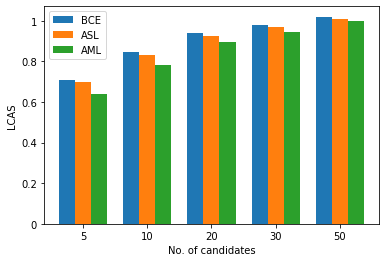
\includegraphics[width=.6\textwidth]{figures/evaluation/all_lcas.png}
    \caption{LCAS comparison of the three models.}
    \label{fig:all_lcas}
\end{figure}